\documentclass[10 pt]{article}
\usepackage[utf8]{inputenc}
\usepackage{amsmath,amssymb,amsthm,tabu,enumerate,tikz}
\usepackage[margin=.25in]{geometry}
\usepackage{verbatim} % Allows Multi-line comments 
\usepackage{multicol}
\usetikzlibrary{calc, shapes, backgrounds}
\usetikzlibrary{automata,positioning}
\newcommand{\encode}[1]{\langle #1 \ra\usetikzlibrary{calc, shapes, backgrounds}ngle}
\usepackage{hyperref}
\usepackage{paralist}
  \let\enumerate\compactenum
  
\setlength{\parskip}{0cm}

\title{350StudyGuide}
\author{David Cobbley }
\date{March 2015}

\begin{document}

\maketitle

\tableofcontents
\pagebreak
\section{Review elementary modular arithmetic}
aka congruences
$a$ is congruent to $b$ mod $m$ iff m divides (a-b) with no remainder. $\beta b(mod (m))$

Reflexive: $a \beta a(mod(m))$ iff $a$ is an integer.

Symmetric: Iff $a \beta b(mod(m))$ then $b \beta a(mod(m))$

Transitive: Iff $a \beta b(mod (m))$ and $ b \beta c(mod(m))$ then $a \beta c(mod(m))$.





% Website links
\href{http://www.articlesforeducators.com/article.asp?aid=161#.VQTEfY7F_iU}{Congruences Link 1}

\href{http://mathworld.wolfram.com/Congruence.html}{Congruences Link 2}

\section{Review induction proofs}


\section{Review Master method}
For $T(n) \leq aT (\frac{n}{b}) + O(n^d)$

Case 1. $O(n^d log(n))$ if $a = b^d$

Case 2. $O(n^d)$ if $a < b^d$

Case 3. $O(n^{log_b a})$ if $a>b^d$ 


\section{Basic facts about binary representation and geometric series}

\begin{multicols}{2}
Gemoetric progression is a sequence of numbers where each term after the first is found by multiplying the previous one by a fixed, non-zero number called the common ratio. For example, the sequence 2, 6, 18, 54, ... is a geometric progression with common ratio 3. Similarly 10, 5, 2.5, 1.25, ... is a geometric sequence with common ratio $\frac{1}{2}$

$1 + 2 + 2^2 + \cdot \cdot \cdot 2^k = \frac{2^{k+1}-1}{2-1} = 2^{k+1}-1$

$1+a+a^2+ \cdot  \cdot  \cdot + a^k = \frac{a^{k+1}-1}{a-1}$

\begin{proof} 
$s_k=1+a+\cdot \cdot \cdot a^k$

$a \cdot  s_k=a+\cdot \cdot \cdot +a^k+a^{k+1}$

$a \cdot s_k -s_k = a^{k+1}-1$

$(a-1) s_k = a^{h+1} -a$

$s_k = \frac{a^{k+1}-1}{a-1} = \frac{k+1}{1} = k+1$
\end{proof}
If $a<1$ $k \rightarrow \frac{infty -1}{a-1} = \frac{1}{1-a}$

\href{http://stackoverflow.com/questions/2126031/converting-a-repeating-binary-number-to-decimal-express-as-a-series}{Geo Series - stack overflow}

\end{multicols}
\section{Review binomial coefficients}
Factorial formula
$n \choose k$ $\rightarrow$ $\frac{n!}{k!(n-k)!}$

Recursive
$n \choose k$ = $ {n-1} \choose {k-1}$ $+$ ${n-1} \choose k$ For all int $n,k:1 \leq k \leq n-1$

Multiplicative
$n \choose k$ = $\frac{n^k}{k!} = \frac{n(n-1)(n-2) \cdot \cdot \cdot (n-(k-1))}{k(k-1)(k-2)\cdot \cdot \cdot 1} = \Pi_{i=1}^k \frac{n-(k-i)}{i} = \Pi_{i=1}^k \frac{n+1-i}{i}$


\href{http://en.wikipedia.org/wiki/Binomial_coefficient}{binomial coeff - wiki}
\section{Review asymptotic notations}

Big-O: Ceiling / Worst case

Little-O: Floor but doesn't touch

Big-Theta: f(n) Bounded above and below by g(n). Basically two big o's - known range of constants.

Big-Omega: Bounded below. Takes x amount of time.


\section{Review spanning tree and MST concepts}
Given a connected, undirected graph. a spanning tree of that graph is a subgraph that is a tree and connects all the vertices together. A single graph can have many different spanning trees. We can also assign a weight to each edge, which is a number representing how unfavorable it is, and use this to assign a weight to a spanning tree by computing the sum of the weights of the edges in that spanning tree. A minimum spanning tree (MST) or minimum weight spanning tree is then a spanning tree with weight less than or equal to the weight of every other spanning tree. More generally, any undirected graph (not necessarily connected) has a minimum spanning forest, which is a union of minimum spanning trees for its connected components.

Uniqueness: If the edge weights are not unique, only the (multi-)set of weights in minimum spanning trees is unique, that is the same for all minimum spanning trees.

\begin{proof}
\item Assume the contrary, that there are two different msts A and B.
\item Let e1 be the edge of least weight that is in one of the MSTs and not the other. Without loss of generality, assume e1 is in A but not in B.
\item As B is a mst, e1 $\cup$ B must contain a cycle C.
\item Then C has an edge e2 whose weight is greater than the weight of e1, since all edges in B with less weight are in A by the choice of e1, and C must have at least one edge that is not in A because otherwise A would contain a cycle in contradiction with its being an MST.
\item Replacing e2 with e1 in B yields a spanning tree with a smaller weight.
\item This contradicts the assumption that B is a MST.
\end{proof}

Minimum cost subgraph: If the weights are positive, then a minimum spanning tree is in fact a minimum-cost subgraph connecting all vertices, since subgraphs containing cycles necessarily have more total weight.

Cycle property: For any cycle C in the graph, if the weight of an edge e of C is larger than the weights of all other edges of C, then this edge cannot belong to a MST.

Cut property: For any cut C in the graph, if the weight of an edge e of C is strictly smaller than the weights of all other edges of C, then this edge belongs to all MSTs of the graph.

Minimum-cost edge: If the edge of a graph with the minimum cost e is unique, then this edge is included in any MST.

Proof: if e was not included in the MST, removing any of the (larger cost) edges in the cycle formed after adding e to the MST, would yield a spanning tree of smaller weight.

\textbf{spanning tree} T of an undirected graph G is a subgraph that includes all of the vertices of G that is a tree. In general, a graph may have several spanning trees, but a graph that is not connected will not contain a spanning tree (but see Spanning forests below). If all of the edges of G are also edges of a spanning tree T of G, then G is a tree and is identical to T (that is, a tree has a unique spanning tree and it is itself).

A tree is a connected undirected graph with no cycles. It is a spanning tree of a graph G if it spans G (that is, it includes every vertex of G) and is a subgraph of G (every edge in the tree belongs to G). A spanning tree of a connected graph G can also be defined as a maximal set of edges of G that contains no cycle, or as a minimal set of edges that connect all vertices.

\section{Review FWK algorithm and least cost paths}
Shortest path for pos/neg weighted graph. no negative cycles. 
one run through the graph will return the summed weights of the shortest path between all pairs of vertices. 

\begin{verbatim}
1 let dist be a |V| x |V| array of minimum distances initialized to infinity
2 for each vertex v
3    dist[v][v] <- 0
4 for each edge (u,v)
5    dist[u][v] <- w(u,v)  // the weight of the edge (u,v)
6 for k from 1 to |V|
7    for i from 1 to |V|
8       for j from 1 to |V|
9          if dist[i][j] > dist[i][k] + dist[k][j] 
10             dist[i][j] <- dist[i][k] + dist[k][j]
11         end if
\end{verbatim}

Bellman–Ford algorithm is an algorithm that computes shortest paths from a single source vertex to all of the other vertices in a weighted digraph.[1] It is slower than Dijkstra's algorithm for the same problem, but more versatile, as it is capable of handling graphs in which some of the edge weights are negative numbers.

\begin{verbatim}
function BellmanFord(list vertices, list edges, vertex source)
   ::distance[],predecessor[]
   // This implementation takes in a graph, represented as
   // lists of vertices and edges, and fills two arrays
   // (distance and predecessor) with shortest-path
   // (less cost/distance/metric) information
   // Step 1: initialize graph
   for each vertex v in vertices:
       if v is source then distance[v] := 0
       else distance[v] := inf
       predecessor[v] := null

   // Step 2: relax edges repeatedly
   for i from 1 to size(vertices)-1:
       for each edge (u, v) with weight w in edges:
           if distance[u] + w < distance[v]:
               distance[v] := distance[u] + w
               predecessor[v] := u

   // Step 3: check for negative-weight cycles
   for each edge (u, v) with weight w in edges:
       if distance[u] + w < distance[v]:
           error "Graph contains a negative-weight cycle"
   return distance[], predecessor[]
\end{verbatim}

Dijkstras For a given source node in the graph, the algorithm finds the shortest path between that node and every other.It can also be used for finding the shortest paths from a single node to a single destination node by stopping the algorithm once the shortest path to the destination node has been determined. For example, if the nodes of the graph represent cities and edge path costs represent driving distances between pairs of cities connected by a direct road.

Assign to every node a tentative distance value: set it to zero for our initial node and to infinity for all other nodes.
Set the initial node as current. Mark all other nodes unvisited. Create a set of all the unvisited nodes called the unvisited set.
For the current node, consider all of its unvisited neighbors and calculate their tentative distances. Compare the newly calculated tentative distance to the current assigned value and assign the smaller one. For example, if the current node A is marked with a distance of 6, and the edge connecting it with a neighbor B has length 2, then the distance to B (through A) will be 6 + 2 = 8. If B was previously marked with a distance greater than 8 then change it to 8. Otherwise, keep the current value.
When we are done considering all of the neighbors of the current node, mark the current node as visited and remove it from the unvisited set. A visited node will never be checked again.
If the destination node has been marked visited (when planning a route between two specific nodes) or if the smallest tentative distance among the nodes in the unvisited set is infinity (when planning a complete traversal; occurs when there is no connection between the initial node and remaining unvisited nodes), then stop. The algorithm has finished.
Select the unvisited node that is marked with the smallest tentative distance, and set it as the new "current node" then go back to step 3.

\section{Review basic facts about polynomial arithmetic and interpolation}
A circle needs 3 pts, a line needs 2 points(has a degree of one).

Given a set of n+1 (xi,yi) where no two xxi are the same, one is looking for a polynomial p of degree at most n with the property: p(xi)=yi, i=0...n

Ex: p(x) = 1+3x+$2x^3$ 
p(1)... 
p(2)

equivalent if null space is zero.

\section{Complexity class def. \& PTIME reducibility def. \& elementary properties}

\section{Greedy Algorithms}
We can make whatever choice seems best at the moment and then solve the subproblems that arise later. The choice made by a greedy algorithm may depend on choices made so far but not on future choices or all the solutions to the subproblem. It iteratively makes one greedy choice after another, reducing each given problem into a smaller one. In other words, a greedy algorithm never reconsiders its choices. This is the main difference from dynamic programming, which is exhaustive and is guaranteed to find the solution. After every stage, dynamic programming makes decisions based on all the decisions made in the previous stage, and may reconsider the previous stage's algorithmic path to solution.

characterized as being 'short sighted', and also as 'non-recoverable'. 

\section{Prims algorithm}
a greedy algorithm that finds a minimum spanning tree for a connected weighted undirected graph. This means it finds a subset of the edges that forms a tree that includes every vertex, where the total weight of all the edges in the tree is minimized
\begin{enumerate}
\item Initialize a tree with a single vertex, chosen arbitrarily from the graph.
\item Grow the tree by one edge: of the edges that connect the tree to vertices not yet in the tree, find the minimum-weight edge, and transfer it to the tree.
\item Repeat step 2 (until all vertices are in the tree).

\end{enumerate}

Time complexity:
In the method that uses binary heaps, we can observe that the traversal is executed O(V+E) times (similar to BFS). Each traversal has operation which takes O(LogV) time. So overall time complexity is O(E+V)*O(LogV) which is O((E+V)*LogV) = O(E*LogV) (For a connected graph, V = O(E)).

\section{Kruskals}
MST for a connected weighted graph. If the graph is not connected, then it finds a minimum spanning forest (a minimum spanning tree for each connected component).

Algorithm:
\begin{enumerate}
\item create a forest F (a set of trees), where each vertex in the graph is a separate tree
\item create a set S containing all the edges in the graph
\item while S is nonempty and F is not yet spanning
    
    -remove an edge with minimum weight from S
    
    -if that edge connects two different trees, then add it to the forest F, combining two trees into a single tree
\end{enumerate}

At the termination of the algorithm, the forest forms a minimum spanning forest of the graph. If the graph is connected, the forest has a single component and forms a minimum spanning tree.


\section{Dynamic Programming}
Solving by breaking down into a collection of simpler subproblems.

Should have bigger sub problems, and smaller ones.
Start with the smallest. Calculating the sum of the weights in a graph. Start calculating the weights at the bottom. Then add that sum to the next weight up instead of recalculating....

\section{Knapsack}

\begin{multicols}{2}
The knapsack problem or rucksack problem is a problem in combinatorial optimization: Given a set of items, each with a mass and a value, determine the number of each item to include in a collection so that the total weight is less than or equal to a given limit and the total value is as large as possible. It derives its name from the problem faced by someone who is constrained by a fixed-size knapsack and must fill it with the most valuable items.


Greedy Continuous-Knapsack$(w,v,W)$
\begin{enumerate}
\item FOR $i=1$ to $n$
\item \hspace{10pt} do $x[i] = 0$
\item $weight = 0$
\item While $weight < W$
\item \hspace{10pt} do $i = $best remaining item
\item \hspace{20pt} IF $weight + w[i] \leq W$
\item \hspace{30pt} then $x[i] = 1$
\item \hspace{40pt} $weight = weight + w[i]$
\item \hspace{30pt} else
\item \hspace{40pt} $x[i] = (w-weight) \backslash w[i]$
\item \hspace{40pt} $weight = W$
\item return $x$
\end{enumerate} \hfill \break
The main parts of this algorithm are to:
\begin{enumerate}
\item Get the ratio of each value per weight.
\item sort them
\item Fill Knapsack
\end{enumerate} 

We know $n^{O(1)} \equiv O(e^n)$

\end{multicols}
\section{Travelling Salesman}
The travelling salesman problem (TSP) asks the following question: Given a list of cities and the distances between each pair of cities, what is the shortest possible route that visits each city exactly once and returns to the origin city? It is an NP-hard problem in combinatorial optimization, important in operations research and theoretical computer science.

Solution of a travelling salesman problem
TSP is a special case of the travelling purchaser problem.

In the theory of computational complexity, the decision version of the TSP (where, given a length L, the task is to decide whether the graph has any tour shorter than L) belongs to the class of NP-complete problems. Thus, it is possible that the worst-case running time for any algorithm for the TSP increases superpolynomially (or perhaps exponentially) with the number of cities.

\section{Halting Problem}
the halting problem is the problem of determining, from a description of an arbitrary computer program and an input, whether the program will finish running or continue to run forever

\section{Np hard vs complete}
P: A decision problem that can be solved in polynomial time. That is, given an instance of the problem, the answer yes or no can be decided in polynomial time.

Example: Given a graph connected G, can its vertices be colored using two colors so that no edge is monochromatic. Algorithm: start with an arbitrary vertex, color it red and all of its neighbors blue and continue. Stop when you run our of vertices or you are forced to make an edge have both of its endpoints be the same color.

NP: A decision problem where instances of the problem for which the answer is yes have proofs that can be verified in polynomial time. This means that if someone gives us an instance of the problem and a certificate (sometimes called a witness) to the answer being yes, we can check that it is correct in polynomial time.

Example: Integer factorization is NP. This is the problem that given integers n and m, is there an integer f with 1 < f < m such that f divides n (f is a small factor of n)? This is a decision problem because the answers are yes or no. If someone hands us an instance of the problem (so they hand us integers n and m) and an integer f with 1 < f < m and claim that f is a factor of n (the certificate) we can check the answer in polynomial time by performing the division n / f.

NP-complete: An NP problem X for which it is possible to reduce any other NP problem Y to X in polynomial time. Intuitively this means that we can solve Y quickly if we know how to solve X quickly. Precisely, Y is reducible to X if there is a polynomial time algorithm f to transform instances y of Y to instances x = f(y) of X in polynomial time with the property that the answer to y is yes if and only if the answer to f(y) is yes.

NP-hard: Intuitively these are the problems that are even harder than the NP-complete problems. Note that NP-hard problems do not have to be in NP (they do not have to be decision problems). The precise definition here is that a problem X is NP-hard if there is an NP-complete problem Y such that Y is reducible to X in polynomial time. But since any NP-complete problem can be reduced to any other NP-complete problem in polynomial time, all NP-complete problems can be reduced to any NP-hard problem in polynomial time. Then if there is a solution to one NP-hard problem in polynomial time, there is a solution to all NP problems in polynomial time.

The halting problem is the classic NP-hard problem. This is the problem that given a program P and input I, will it halt? This is a decision problem but it is not in NP. It is clear that any NP-complete problem can be reduced to this one.

P = NP: This the most famous problem in computer science, and one of the most important outstanding questions in the mathematical sciences. In fact, the Clay Institute is offering one million dollars for a solution to the problem (Stephen Cook's writeup on the Clay website is quite good). It's clear that P is a subset of NP. The open question is whether or not NP problems have deterministic polynomial time solutions. It is largely believed that they do not. Here is an outstanding recent article on the latest (and the importance) of the P = NP problem: 


\section{Decidable vs undecidable}
A TM recognizes a language if it accepts all
and only those strings in the language
A TM decides a language if it accepts all
strings in the language and rejects all strings
not in the language
A language is called recognizable or
recursively enumerable, (or r.e.)
if some TM recognizes it
A language is called decidable (or recursive)
if some TM decides it

\section{Logs}

\begin{multicols}{2}
logb(mn) = logb(m) + logb(n)

2) logb(m/n) = logb(m) – logb(n)

3) logb(mn) = n · logb(m)

In less formal terms, the log rules might be expressed as:

1) Multiplication inside the log can be turned into addition outside the log, and vice versa.

2) Division inside the log can be turned into subtraction outside the log, and vice versa.

3) An exponent on everything inside a log can be moved out front as a multiplier, and vice versa.



log3(2x) = log3(2) + log3(x) is log3(2) + log3(x)
Expand log4( 16/x ).
log4( 16/x ) = log4(16) – log4(x)
log4(16) = 2
log4( 16/x ) = 2 – log4(x)

Expand log5(x3).  
log5(x3) = 3 · log5(x) = 3log5(x)

\end{multicols}

\section{p-time}
a polynomial-time reduction is a method of solving one problem by means of a hypothetical subroutine for solving a different problem (that is, a reduction), that uses polynomial time excluding the time within the subroutine. There are several different types of polynomial-time reduction, depending on the details of how the subroutine is used. Intuitively, a polynomial-time reduction proves that the first problem is no more difficult than the second one, because whenever an efficient algorithm exists for the second problem, one exists for the first problem as well. Polynomial-time reductions are frequently used in complexity theory for defining both complexity classes and complete problems for those classes.

\subsection{completeness}
A complete problem for a given complexity class C and reduction $\leq$ is a problem P that belongs to C, such that every problem A in C has a reduction A $\leq$ P. For instance, a problem is NP-complete if it belongs to NP and all problems in NP have polynomial-time many-one reductions to it. A problem that belongs to NP can be proven to be NP-complete by finding a single polynomial-time many-one reduction to it from a known NP-complete problem.[4] Polynomial-time many-one reductions have been used to define complete problems for other complexity classes, including the PSPACE-complete languages and EXPTIME-complete languages.

Every decision problem in P (the class of polynomial-time decision problems, where nontrivial means that not every input has the same output) may be reduced to every other nontrivial decision problem, by a polynomial-time many-one reduction. To transform an instance of problem A to B, solve A in polynomial time, and then use the solution to choose one of two instances of problem B with different answers. Therefore, for complexity classes within P such as L, NL, NC, and P itself, polynomial-time reductions cannot be used to define complete languages: if they were used in this way, every nontrivial problem in P would be complete. Instead, weaker reductions such as log-space reductions or NC reductions are used for defining classes of complete problems for these classes, such as the P-complete problems.[6]

\section{permutations}
The resulting algorithm for generating a random permutation of a[0], a[1], ..., a[n - 1] can be described as follows in pseudocode:
\begin{verbatim}

for i from n downto 2
do   di $<-$ random element of { 0, ..., i - 1 }
swap a[di] and a[i - 1]
This can be combined with the initialization of the array a[i] = i as follows:

for i from 0 to n-1
do   di+1 $<-$ random element of { 0, ..., i }
a[i] $<-$ a[di+1]
a[di+1] $<-$ i
If di+1 = i, the first assignment will copy an uninitialized value, 
but the second will overwrite it with the correct value i.

\end{verbatim}

\section{Huffman}

\begin{multicols}{2}
The simplest construction algorithm uses a priority queue where the node with lowest probability is given highest priority:

Create a leaf node for each symbol and add it to the priority queue.
While there is more than one node in the queue:
Remove the two nodes of highest priority (lowest probability) from the queue
Create a new internal node with these two nodes as children and with probability equal to the sum of the two nodes' probabilities.
Add the new node to the queue.
The remaining node is the root node and the tree is complete.
Since efficient priority queue data structures require O(log n) time per insertion, and a tree with n leaves has 2n-1 nodes, this algorithm operates in O(n log n) time, where n is the number of symbols.

Data: takes a frequency table

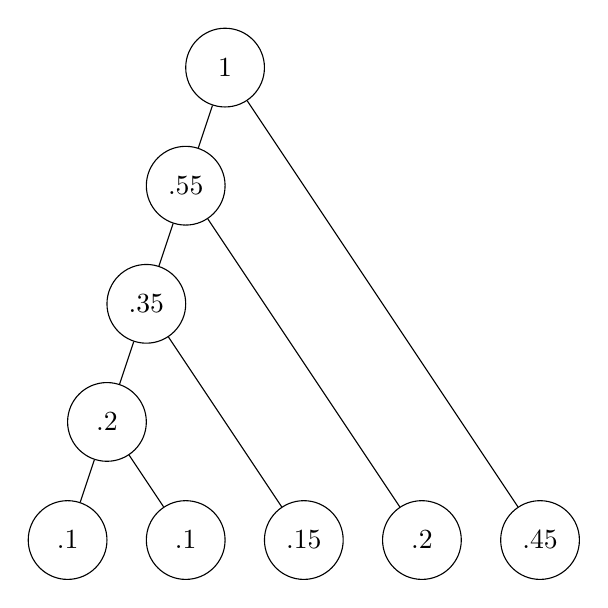
\begin{tikzpicture}[every node/.style = {draw, circle, minimum size = 10mm}]

  \node (a) at (0,0) {.1};
  \node (b) at (1.5,0) {.1};
  \node (c) at (3,0) {.15};
  \node (d) at (4.5,0) {.2};
  \node (e) at (6,0) {.45};
  \node (f) at (.5,1.5) {.2};
  \node (g) at (1,3) {.35};
  \node (h) at (1.5,4.5) {.55};
  \node (i) at (2,6) {1};
  
  
  \draw (a)--(f)--(b) (f)--(g)--(c) (g)--(h)--(d) (h)--(i)--(e) ; 
  %\draw (a)--(b) (a)--(c)--(d) (c)--(e);
\end{tikzpicture}

\end{multicols}
\section{other algorithms}
LCS:


$LCS[i,j]$ is the length of the LCS of $S[1..j]$ with $T[1..j]$

Two cases for the LCS:
\begin{enumerate}
\item If $S[i] \not = T[j]$ then:

\hspace{35pt} $LCS[i,j] = max(LCS[i - 1,j], LCS[i,j-1])$

\item If $S[i] = T[j]:$

\hspace{35pt} $LCS[i,j] = 1 + LCS[i-1,j-1]$.
\end{enumerate} \hfill \break


MST uniqueness:

Prove that a graph with a distinct weight for each edge has a unique MST.
%http://ocw.mit.edu/courses/electrical-engineering-and-computer-science/6-046j-design-and-analysis-of-algorithms-spring-2012/lecture-notes/MIT6_046JS12_lec03.pdf

\begin{proof} \textit{by contradiction}

Assume that if an edge is the unique light edge on a cut, it must be in every MST of G. \hfill \break

Let $T$ be an MST of $G$. Assume that $T'$ is a different MST of $G$. $T$ and $T'$ both have edges $|V|-1$. There exists some edge $e$ in $T$ that is not in $T'$. Removing $e$ from $T$ creates a new cut of $G$. 
Because $T$ is a spanning tree, removing $e$ divides $G$ into two disjoint sets of vertices, together they include all vertices of $G$. Now, since $T$ is an MST, $e$ must be the unique light edge and is in every MST. Edge $e$ is not in $T'$. Therefore $T'$ is not an MST.
\end{proof}


Using the Knuth-Morris-Pratt matching algorithm$(T,P)$
\begin{enumerate}
\item $n= T.length$
\item $m = P.length$
\item $\pi = COMPUTE-PREFIX-FUNCTION(P)$
\item $q = 0$
\item \textbf{for} $i = 1$ \textbf{to} $n$
\item \hspace{10pt} \textbf{while} $q > 0$ and $P[q+1] \not = T[i]$
\item \hspace{20pt} $q = \pi [q]$
\item \hspace{10pt} \textbf{if} $P[q+1] == T[i]$
\item \hspace{20pt} $q = q + 1$
\item \hspace{10pt} \textbf{if} $q == m$
\item \hspace{20pt} print "Patern occurs with shift" $i-m$
\item \hspace{20pt} $q = \pi[q]$
\end{enumerate}\hfill \break 

Time Complexity $O(n)$

\paragraph{Extras}
FWK- Adapart it to accumulate a set of every vertex reachable from the current place instead of incrementing a counter for each vertex that is the set of all reachable vertexes starting from [i,s]. If diagonal contains vertex and inverse, not satisfiable.



mst with one path that isn't the least cost

\section{midterm solutions}

\paragraph{1} Let $G=(V,E)$ be a DAG
\begin{enumerate}
\item Give an example of a DAG with a topological sort in which for some vertices $i < j, (i,j) \not \in E$.
Let $G=(V,E)$ where the topologically sorted $V = \{1,2\}$ and $ E = \emptyset$.
\item Determine the max num edges in a DAG with V vertices.
Claim: max size $E$ is $\frac{(V-1) \cdot V}{2}$ To see this lay out the vertices 1,2,...V and include every edge(i,j) for $i<j$. The count is just V-1+...+1.
\end{enumerate}
\paragraph{2}Give an algorithm based on DFS to determine whether a digraph is strongly connected
Run $DFS(G,v)$p for each v and check that each search tree contains all of V. 
G is a single SCC $\Leftrightarrow$ each tree contains V.
\paragraph{3}Determine which master method case if any: 
$T(n) = 5 \cdot T(n/3) + \frac{n^{\frac{4}{3}} }{log(n)}$

Here a = 5 and b = 3 so look at $log_b a = log _3 5$.
Because $log_3 5 > \frac{4}{3}$ because $3^{3 \cdot log_3 5} = 5^3 > 3^4$

This yields case 1 $T(n) = \Theta (n^{log_3 5})$.
\paragraph{4}Prove that if $j<i\leq \lfloor \frac{n}{2} \rfloor$, Then ${n \choose j} < {n \choose i}$
Show it for $j=i-1$ and use transitivity of $<$.

${n \choose i} < {n \choose i+1}$ subject to $i+1 \leq \lfloor \frac{n}{2} \rfloor$

The case $i=0$ is clear so we assume $i>0$ From the definition

$n \choose i = \frac{ n \cdot \cdot \cdot (n-(i-1))}{i!}$

and

$n \choose i+1 = \frac{ n \cdot \cdot \cdot (n-(n-i))}{(i+1)!}$

cross multiply and we get

$i +1 :: n-i$ But $i < \frac{n-1}{2}$ because $ i+1 \leq \lfloor \frac{n}{2} \rfloor$
\paragraph{5} Let G be a tree (connected, acyclic graph). Show that there is exactly one path between any two distinct vertices's. Assume there are two paths between two vertices and show that a cycle must exist.

Assume there are two paths $\alpha$ and $\beta$ between $x$ and $y$. There must be two vertices $u$ and $v$ that are both on $\alpha$ and $\beta$ but so that the sets of vertices on the subpaths of $\alpha$ and $\beta$ between $u$ and $v$ are disjoint. But this yields a cycle... Contradiction.

\paragraph{6}
\begin{enumerate}
\item Show that a permutation cycle $\sigma = (i_1 \cdot \cdot \cdot i_r)$ satisfies $ \sigma^r = (i_1) \cdot \cdot \cdot (i_r)$. 

We know that $\sigma^r$ sends $i_j$ to $i_j+r$ mod $r$ but j+ r mod r = j, that is $\sigma^r$ sends $i_j$ to $ i_j$.

\item Assume part 1. Let the permutation $\tau$ act on [0...n-1] have a disjoint cycle factorization $\tau_1 \cdot \cdot \cdot \tau_s$, where $\tau_i$ is a cycle of length $k_i$. Show that 

$\tau^{k_1 \cdot \cdot \cdot k_s} = (0)(1) \cdot \cdot \cdot (n-1)$

Since the cycles $\tau_1,....., \tau_s$ are disjoint,

$\tau^{k_1 \cdot \cdot \cdot k_s} = \tau_1^{k_1 \cdot \cdot \cdot k_s} \cdot \cdot \cdot \tau_s^{k_1 \cdot \cdot \cdot k_s}$

From part 1, $\tau_i^{k_i}$ is the identity permutation. Any power of $\tau_i^{k_i}$ is still the identity. It follows that 

$(\tau_i^{k_i})^{\frac{k_1...k_s}{k_i}} = \tau_i^{k_1...k_s}$

is the identity so then is $\tau^{k_1...k_s}$. 

\end{enumerate}

\begin{multicols}{2}
\paragraph{7} Recall that $\frac{1}{x \cdot (x+1} = \frac{1}{x} - \frac{1}{x+1}$

Use this to prove that for $n \geq 1$

$\sum\limits_{i=1}^n \frac{1}{i \cdot (i+1)} = \frac{n}{n+1}$

Proof1 induction. Basis $n=1$ checks since $\frac{1}{2}=\frac{1}{2}$

Induction: Assume

$\sum\limits_{i=1}^n \frac{1}{i \cdot (i+1)} = \frac{n}{n+1}$

Thus
$\sum\limits_{i=1}^n \frac{1}{i \cdot (i+1)} = \frac{n}{n+1}+ \frac{1}{(n+1) \cdot (n+2)}$

One checks that 
$\frac{n}{n+1}+ \frac{1}{(n+1) \cdot (n+2)} = \frac{n+1}{n+2}$

Proof 2. Partial fracs

$\sum\limits_{i=1}^n \frac{1}{i \cdot (i+1)} =\sum\limits_{i=1}^n \frac{1}{i} - \sum\limits_{j=1}^n \frac{1}{j+1}$

After cancelling like terms we get 

$1- \frac{1}{n+1}= \frac{n}{n+1}$


More extras:
 Convert the Euclidean GCD algorithm to an iterative version. Analyze your algorithm: termination, correctness and running time.

\begin{verbatim}
GCD(i,j)
int k
while(j!=0)
    k=i
    i=j
    j=i mod j
if i<0 
    return  -i \\fail
else
    return i
\end{verbatim}



\paragraph{Problem 1} Use the fact that for $n > 2$, \hfill \\
$2 < (1 + \frac{1}{n})^n < 3$\\
to prove by induction that \hfill \\
$\frac{n^n}{3^n} < n! < \frac{n^n}{2^n}$.

\begin{proof}
$2 < (1 + \frac{1}{n})^n < 3$
Base(p(n=3))\\
$2<(1+\frac{1}{n})^n<3$\\
$2<(\frac{n}{n} +\frac{1}{n})^n<3$\\
$2<(\frac{n+1}{n})^n<3$\\
$\frac{1}{2} > (\frac{n}{n+1})^n > \frac{1}{3}$
\end{proof}

\begin{proof} Base(p(n=6))

$\frac{6^6}{3^6} < 6! < \frac{6^6}{2^6}$ 
= $64 < 720 < 729$.
True \checkmark.

Induction:

Now (p(n+1)). $\frac{n+1^{n+1}}{3^{n+1}}$ $<$ $(n+1)!$ $<$ $\frac{n+1^{n+1}}{2^{n+1}}$.

Expand the left hand side.

$\frac{1}{3} * \frac{k+1^{k+1}}{3^k} * (k+1)
= \frac{1}{3}*\big( \frac{k+1}{3} \big) ^k (k+1)$. 

$=(k+1)*\frac{k+1^k}{3^k} < k! < (k+1)!$

$=\big(\frac{k}{k+1} * \frac{k+1}{3}\big) ^k * (k+1) < (k+1)!$

$=\big( \frac{k}{k+1} \big(^k * \big(\frac{k+1}{3}\big)^3 (k+1) < (k+1)!$

$\therefore$ by the property of transitivity, $\frac{k+1^{k+1}}{3^{k+1}} < (k+1)!$

\vspace{10pt}
Expand the right hand side - prove $(k+1)!< \frac{k+1^{k+1}}{2^{k+1}}$.

We know that $\frac{k+1^{k+1}}{2^{k+1}}$ is equivalent to $\frac{1}{2} * \frac{k+1}{2} * (k+1)$

$k! < \frac{k^k}{2^k}$ for $k \geq 6$.


$(k+1)! < (\frac{k}{k+1} * \frac{k+1}{2})^2 (k+1)$.

$(k+1)! < (\frac{k}{k+1})^k * (\frac{k+1}{2})^k * (k+1)$.

$(\frac{k}{k+1})^k = \frac{1}{2}$ when k = 1.


$(k+1)! < (\frac{k}{k+1})^k (\frac{k+1}{2}) (k+1) < \frac{1}{2} (\frac{k+1}{2})^k (k+1)  -> (\frac{k}{k+1})^k < \frac{1}{2}$.


By the property of transitivity, $(k+1)! < \frac{k+1^{k+1}}{2^{k+1}}$.

$\frac{k+1^{k+1}}{3^{k+1}} < (k+1)! < \frac{k+1}{2^{k+1}}$.

Therefore $\frac{n^n}{3^n} < n! < \frac{n^n}{2^n}$ holds true.

\end{proof}
\end{multicols}
\begin{comment}
\section{Left to study}

DFS VS BFS

Bellman vs Dijkstra

Dynamic Programming

big o cheat sheet
\end{comment}
\end{document}

